\documentclass[10pt,twocolumn]{article}
\usepackage[utf8]{inputenc}
\usepackage[margin=0.75in]{geometry}
\usepackage{graphicx}
\usepackage{tikz}
\usepackage{xcolor}
\usepackage{fontspec}
\usepackage{microtype}
\usepackage{titlesec}
\usepackage{fancyhdr}
\usepackage{abstract}
\usepackage{lettrine}

% Color scheme
\definecolor{gardengreen}{RGB}{74,124,58}
\definecolor{serpentgold}{RGB}{212,175,55}
\definecolor{edengray}{RGB}{85,85,85}
\definecolor{fallred}{RGB}{180,50,50}
\definecolor{wisdomblue}{RGB}{70,130,180}

% Font setup
\setmainfont{Times New Roman}
\setsansfont{Arial}

% Title formatting
\titleformat{\section}{\Large\bfseries\color{gardengreen}}{\thesection}{1em}{}
\titleformat{\subsection}{\large\bfseries\color{edengray}}{\thesubsection}{1em}{}

% Header/footer
\pagestyle{fancy}
\fancyhf{}
\fancyhead[LE,RO]{\color{gardengreen}\small\textit{The Serpent's Sentence}}
\fancyhead[RE,LO]{\color{edengray}\small Justin T. Bogner}
\fancyfoot[C]{\color{gardengreen}\thepage}
\renewcommand{\headrulewidth}{0.4pt}
\renewcommand{\headrule}{\hbox to\headwidth{\color{gardengreen}\leaders\hrule height \headrulewidth\hfill}}

% Abstract styling
\renewcommand{\abstractname}{\color{gardengreen}Abstract}

% Language evolution timeline
\newcommand{\languagetimeline}{
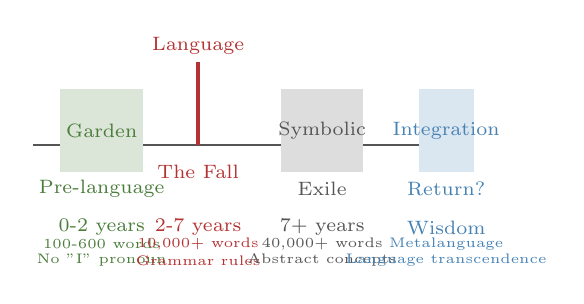
\begin{tikzpicture}[scale=0.7]
    % Timeline arrow
    \draw[edengray, thick, ->] (0,0) -- (8,0);
    
    % Pre-language (Garden)
    \fill[gardengreen!20] (0.5,-0.5) rectangle (2,1);
    \node[gardengreen, font=\scriptsize] at (1.25,0.25) {Garden};
    \node[gardengreen, font=\scriptsize] at (1.25,-0.8) {Pre-language};
    
    % Language emergence (Fall)
    \draw[fallred, very thick] (3,0) -- (3,1.5);
    \node[fallred, font=\scriptsize] at (3,1.8) {Language};
    \node[fallred, font=\scriptsize] at (3,-0.5) {The Fall};
    
    % Symbolic consciousness (Exile)
    \fill[edengray!20] (4.5,-0.5) rectangle (6,1);
    \node[edengray, font=\scriptsize] at (5.25,0.25) {Symbolic};
    \node[edengray, font=\scriptsize] at (5.25,-0.8) {Exile};
    
    % Potential integration (Return)
    \fill[wisdomblue!20] (7,-0.5) rectangle (8,1);
    \node[wisdomblue, font=\scriptsize] at (7.5,0.25) {Integration};
    \node[wisdomblue, font=\scriptsize] at (7.5,-0.8) {Return?};
    
    % Time labels with language acquisition milestones
    \node[gardengreen, font=\scriptsize] at (1.25,-1.5) {0-2 years};
    \node[gardengreen, font=\tiny] at (1.25,-1.8) {100-600 words};
    \node[gardengreen, font=\tiny] at (1.25,-2.1) {No "I" pronoun};
    \node[fallred, font=\scriptsize] at (3,-1.5) {2-7 years};
    \node[fallred, font=\tiny] at (3,-1.8) {10,000+ words};
    \node[fallred, font=\tiny] at (3,-2.1) {Grammar rules};
    \node[edengray, font=\scriptsize] at (5.25,-1.5) {7+ years};
    \node[edengray, font=\tiny] at (5.25,-1.8) {40,000+ words};
    \node[edengray, font=\tiny] at (5.25,-2.1) {Abstract concepts};
    \node[wisdomblue, font=\scriptsize] at (7.5,-1.5) {Wisdom};
    \node[wisdomblue, font=\tiny] at (7.5,-1.8) {Metalanguage};
    \node[wisdomblue, font=\tiny] at (7.5,-2.1) {Language transcendence};
\end{tikzpicture}
}

% Apple of knowledge graphic
\newcommand{\appleknowledge}{
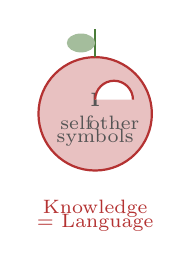
\begin{tikzpicture}[scale=0.6]
    % Apple outline
    \fill[fallred!30] (0,0) circle (1.2);
    \draw[fallred, thick] (0,0) circle (1.2);
    
    % Stem
    \draw[gardengreen, thick] (0,1.2) -- (0,1.8);
    
    % Leaf
    \fill[gardengreen!50] (-0.3,1.5) ellipse (0.3 and 0.2);
    
    % Symbolic content inside apple
    \node[edengray, font=\scriptsize] at (0,0.3) {\textbf{I}};
    \node[edengray, font=\scriptsize] at (-0.4,-0.2) {self};
    \node[edengray, font=\scriptsize] at (0.4,-0.2) {other};
    \node[edengray, font=\scriptsize] at (0,-0.5) {symbols};
    
    % Bite mark
    \fill[white] (0.8,0.3) arc (0:180:0.4);
    \draw[fallred, thick] (0.8,0.3) arc (0:180:0.4);
    
    % Title
    \node[fallred, font=\scriptsize] at (0,-2) {Knowledge};
    \node[fallred, font=\scriptsize] at (0,-2.3) {= Language};
\end{tikzpicture}
}

% Tree of knowledge and life
\newcommand{\twotrees}{
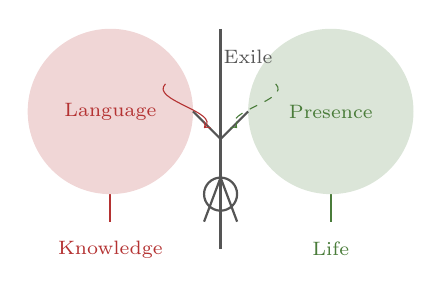
\begin{tikzpicture}[scale=0.7]
    % Tree of Knowledge
    \draw[fallred, thick] (-2,-2) -- (-2,0);
    \fill[fallred!20] (-2,0) circle (1.5);
    \node[fallred, font=\scriptsize] at (-2,-2.5) {Knowledge};
    \node[fallred, font=\scriptsize] at (-2,0) {Language};
    
    % Tree of Life  
    \draw[gardengreen, thick] (2,-2) -- (2,0);
    \fill[gardengreen!20] (2,0) circle (1.5);
    \node[gardengreen, font=\scriptsize] at (2,-2.5) {Life};
    \node[gardengreen, font=\scriptsize] at (2,0) {Presence};
    
    % Human figure between trees
    \draw[edengray, thick] (0,-1.5) circle (0.3);
    \draw[edengray, thick] (0,-1.2) -- (0,0);
    \draw[edengray, thick] (0,-0.5) -- (-0.5,0);
    \draw[edengray, thick] (0,-0.5) -- (0.5,0);
    \draw[edengray, thick] (0,-1.2) -- (-0.3,-2);
    \draw[edengray, thick] (0,-1.2) -- (0.3,-2);
    
    % Choice arrows
    \draw[fallred, ->] (-1,0.5) to[out=225,in=45] (-0.3,-0.3);
    \draw[gardengreen, dashed, ->] (1,0.5) to[out=315,in=135] (0.3,-0.3);
    
    % Wall between trees (exile)
    \draw[edengray, thick] (0,1.5) -- (0,-2.5);
    \node[edengray, font=\scriptsize] at (0.5,1) {Exile};
\end{tikzpicture}
}

\begin{document}

\title{\color{gardengreen}\Huge Language Was Humanity's Fall From Grace}
\author{\color{edengray}\large Justin T. Bogner}
\date{\color{edengray}\today}

\maketitle

\begin{abstract}
The biblical Fall from Eden describes a real cognitive revolution: humanity's transition from pre-linguistic consciousness to symbolic thought. Language gave us civilization, art, and science—but at the cost of direct contact with reality. We traded Paradise for the power to think about Paradise. The question now is whether we can integrate both gifts.
\end{abstract}

\vspace{0.5cm}
\languagetimeline

\lettrine[lines=3]{\color{gardengreen}L}{anguage is humanity's} original sin—not because speaking is evil, but because symbolic thought fundamentally altered our relationship with reality in ways we're only beginning to understand. The moment we learned to represent the world through words, we lost the capacity for direct, unmediated experience that had defined consciousness for millions of years.

This isn't metaphor. It's the literal truth about how language changes the brain, reorganizes perception, and creates the prison of self-consciousness that characterizes human experience. We traded Paradise for the power to think about Paradise—and mostly, we don't even remember what we lost.

The biblical story of the Fall captures this cognitive revolution with startling accuracy. Eden represents pre-linguistic consciousness. The serpent represents the emergence of symbolic thought. The forbidden fruit represents meta-cognitive awareness—the ability to think about thinking. And the exile from Paradise? That's the permanent separation from immediate reality that language imposes on human consciousness.

We gained the ability to manipulate symbols, to transcend our immediate circumstances, to build civilization. But we lost something irreplaceable: the capacity to experience the world directly, without the constant mediation of words, concepts, and the internal narrator that language creates.

This was humanity's Fall from grace. And it happened to you personally, sometime between your second and seventh birthday, when language rewired your brain and locked you out of the Garden forever.

\section{The Garden of Pre-Linguistic Consciousness}

\twotrees

Before you learned to speak—really learned, not just parroted sounds—you lived in a state that mystics have spent lifetimes trying to recover. For the first two years of life, your consciousness was immediate, embodied, and present. You experienced the world directly, without the overlay of concepts that now mediates every perception.

This wasn't a lesser state of consciousness. It was a different kind entirely.

Developmental psychologist Daniel Stern calls this "emergent self" awareness: consciousness that's present and unified but not self-reflective. You could feel pain, pleasure, hunger, comfort, joy, and distress, but you didn't have thoughts \textit{about} these experiences. There was no internal voice commenting on what was happening, no sense of being a separate observer looking out at the world from inside your head.

Brain imaging studies of infants reveal neural activity patterns completely unlike those of language-using adults. The regions that will later support self-referential thinking—the medial prefrontal cortex, posterior cingulate cortex, and angular gyrus—show minimal coordinated activation. Instead, consciousness appears "distributed" across sensory and motor networks without being centralized around a linguistic self-model.

This is exactly what contemplative traditions describe as "original nature" or "Buddha mind": awareness that's present but not personal, conscious but not self-conscious. You lived in this state. You remember none of it, but it was the baseline of human consciousness for millions of years before language arrived.

The Garden of Eden describes this perfectly: a state of immediate presence where humans were "naked and felt no shame"—lacking the symbolic categories that create self-consciousness and separation between self and world.

\section{The Serpent's Gift: Symbolic Cognition}

\appleknowledge

Around age two, something unprecedented began happening in your brain. You started learning that certain sounds could stand for things that weren't present. The sound "mama" could refer to your mother even when she wasn't there. The sound "milk" could represent a liquid you desired. You discovered that reality could be represented symbolically.

This discovery triggered a neural revolution that neuroscientists call "synaptic pruning"—a massive reorganization of brain structure that eliminated millions of connections while strengthening others. The connections that survived were those that supported symbolic cognition: the ability to categorize experience, create mental models, and manipulate abstract representations.

Language acquisition literally requires your brain to abandon vast networks that supported pre-linguistic awareness in favor of new neural highways optimized for symbolic processing. The temporal lobes become dominated by language centers. The frontal cortex develops executive functions that constantly monitor and control experience through linguistic categories.

Most dramatically, language development activates what will become the default mode network—the brain regions that generate the sense of being a separate self existing inside your head, thinking thoughts, having experiences.

The serpent in Eden is described as "more cunning than any beast of the field"—and symbolic cognition is indeed more sophisticated than any other form of animal awareness. Language allows transcendence of immediate circumstance. You can think about the past, imagine the future, contemplate abstract concepts, and coordinate behavior with others across vast scales of space and time.

But this gift comes with a cost that the Eden story makes explicit: once you've eaten from the Tree of Knowledge, you can never return to the Garden of immediate awareness.

\section{The Forbidden Fruit: Meta-Cognitive Awareness}

The Fall doesn't become complete until around age seven, when children develop what psychologists call "theory of mind"—the understanding that they have minds, that others have minds, and that these minds can contain different beliefs, desires, and perspectives.

This is when meta-cognitive awareness emerges: the ability to think about thinking, to model yourself as an object in your own awareness. It's also when the inner critic is born—the constant stream of self-referential commentary that characterizes adult consciousness.

Brain imaging studies show that the default mode network becomes fully active during this developmental period. The medial prefrontal cortex, posterior cingulate cortex, and angular gyrus begin firing together in coordinated patterns that create the experience of being a separate self observing the world.

This network becomes so dominant that most adults spend nearly half their waking hours lost in mental commentary rather than present to immediate experience. The inner voice that seems so natural, so much like the "real you," is actually a late-arriving neural development that fundamentally alters consciousness.

The forbidden fruit represents this meta-cognitive capacity: knowledge of good and evil, self and other, observer and observed. It's the birth of the psychological self that experiences separation from the world it observes.

In the biblical story, eating this fruit makes humans "like God, knowing good and evil." And indeed, meta-cognitive awareness grants god-like powers: the ability to step outside immediate experience, to judge and evaluate, to model multiple perspectives simultaneously.

But it also creates what the story describes as shame: the painful self-consciousness that comes from experiencing yourself as an object that might be found wanting.

\section{Exile from Paradise}

Once symbolic cognition reorganizes your brain, there's no simple path back to pre-linguistic awareness. The neural pathways that supported Garden-state consciousness have been pruned away or integrated into language networks. You become literally exiled from immediate awareness.

This exile isn't punishment—it's the inevitable result of how language changes brain structure. Neuroscientist Lisa Feldman Barrett's research shows that language doesn't just describe reality; it constructs your experience of reality. Once you have words for emotions, sensations, and concepts, your brain automatically uses these linguistic categories to organize all incoming experience.

The result is that you never experience anything directly anymore. Every perception is immediately filtered through language, categorized by concepts, and narrated by the inner voice. Between you and the world stands an impenetrable barrier of words.

This is why meditation traditions emphasize the extraordinary difficulty of accessing what they call "beginner's mind" or "original face." These practices are attempts to temporarily bypass the linguistic processing that normally dominates adult consciousness—to sneak past the "angel with the flaming sword" that guards the entrance to Eden.

But the angel isn't an external force. It's your own brain's automatic tendency to suppress non-linguistic forms of awareness in favor of symbolic processing. The language centers actively inhibit the neural networks that might support pre-linguistic consciousness.

\section{The Price of Symbolic Thought}

Language gave us everything we think of as distinctly human: art, science, philosophy, literature, technology, civilization. The capacity for symbolic thought allows us to transcend animal immediacy, to imagine alternatives to present circumstances, to cooperate across vast scales of space and time.

Without the Fall into language, there would be no human culture. No accumulated knowledge passed between generations. No ability to contemplate abstract concepts like justice, beauty, or truth. No capacity to love someone who isn't physically present or to grieve for the dead.

But the price we paid was the loss of what eco-psychologist David Abram calls "the more-than-human world"—direct sensory contact with a reality that speaks to us without words. Animals still live in this world. Young children live there briefly. But for language-using adults, it remains largely inaccessible.

We gained the ability to think about trees, but we lost the capacity to simply be present with a tree without the mediation of the concept "tree." We can describe the sound of wind, but we rarely hear it directly without the inner voice immediately categorizing the experience.

Most tragically, we gained the ability to think about love, beauty, and meaning, but we largely lost the capacity to experience these realities directly. We live in a world of representations of experience rather than experience itself.

\section{The Neuroscience of Return}

But the Eden story contains a crucial detail that suggests the Fall might not be permanent. After eating from the Tree of Knowledge, humans are expelled from the Garden before they can also eat from the Tree of Life. This implies a form of consciousness that combines symbolic cognition with something else—something that preserves the immediacy and aliveness of pre-linguistic awareness.

Recent neuroscience research suggests this might be more than ancient wishful thinking. The adult brain retains remarkable capacity for structural change through what scientists call "experience-dependent plasticity." Under the right conditions, neural networks can reorganize, potentially creating new possibilities for consciousness.

Studies of advanced contemplatives show unusual patterns of brain connectivity that suggest they've developed what researcher Clifford Saron calls "meta-cognitive balance"—the ability to access both symbolic and pre-symbolic forms of awareness depending on circumstances.

The default mode network in these individuals shows decreased baseline activity but increased flexibility. They can engage symbolic cognition when useful but aren't trapped in it. They seem to have found ways to visit the Garden without abandoning the gifts of knowledge.

Similarly, research on psychedelics, meditation, and other consciousness-altering practices reveals that the brain networks supporting linguistic cognition can be temporarily downregulated, allowing access to forms of awareness that closely resemble pre-linguistic consciousness.

This suggests the possibility of what we might call "post-linguistic consciousness"—awareness that has journeyed through the Fall and found ways to integrate the fruits of both trees.

\section{The Second Garden}

Perhaps the ultimate insight hidden in the Eden story is that Paradise itself evolves. The original Garden was innocent, unconscious, immediate. But the human journey through knowledge and exile might lead to a second Garden: conscious Paradise, awareness that combines innocence with wisdom.

This wouldn't be regression to childhood consciousness. It would be integration: the development of awareness that can move fluidly between symbolic and pre-symbolic modes depending on what each situation requires.

Contemplative traditions have always pointed toward this possibility. Zen's "ordinary mind," Dzogchen's "rigpa," Kashmir Shaivism's "spanda"—these concepts describe awareness that transcends the linguistic self without abandoning cognitive sophistication.

Modern neuroscience is beginning to map how such integration might work. Advanced practitioners seem to develop what could be called "translucent thinking"—the ability to use thoughts and concepts without being trapped by them, to employ symbolic cognition while remaining anchored in immediate presence.

\section{Conscious Evolution Beyond Language}

If language was humanity's Fall from grace, then conscious evolution beyond the limitations of symbolic thought might be our path to redemption. Not by abandoning language—that's impossible and undesirable—but by learning to hold it more lightly.

We can't go back to the original Garden; the neural changes that create symbolic consciousness are irreversible. But we might go forward to a new kind of Paradise: awareness that has journeyed through language and returned home, carrying the fruits of knowledge back to the tree of life.

This would be consciousness that includes but transcends the linguistic self, that can think when thinking is useful but can also access the direct, immediate awareness that language normally obscures.

The question facing humanity now is whether we can accomplish this evolution consciously, as individuals and as a species. Can we learn to integrate the gifts of both trees? Can we develop forms of consciousness that honor both the serpent's wisdom and the Garden's presence?

The stakes are higher than personal liberation. As artificial intelligence develops symbolic cognition that may soon surpass our own, our unique value might lie not in our thinking but in our capacity to bridge symbolic and pre-symbolic awareness, to remain connected to the embodied wisdom that pure symbolic cognition can never access.

We fell into language. Now we must learn to rise into integrated awareness.

The Garden awaits, not behind us in lost innocence, but ahead of us in conscious return. Paradise regained, not through ignorance, but through wisdom that has fully digested the serpent's gift while remembering the tree of life.

\vfill

\begin{center}
\color{gardengreen}\rule{0.5\linewidth}{0.4pt}

\textit{This article is adapted from "The Serpent's Sentence: Language, Consciousness, and the Second Cambrian Mind." For more insights on consciousness and human evolution, visit justintbogner.com}
\end{center}

\end{document}
